\documentclass{article}
\usepackage[utf8]{inputenc}
\usepackage{pifont}
\usepackage{graphicx}
\usepackage{subcaption}
\newcommand{\cmark}{\ding{51}}%
\newcommand{\xmark}{\ding{55}}%

\title{Back-migration V2}
\author{ccole }
\date{January 2020}

\begin{document}

\maketitle

\paragraph{Outline}
\begin{enumerate}
    \item Introduction
    \item Methods
    \item Current Results 
    \begin{enumerate}
        \item Effective population sizes from SMC2 and MSMC, which finds differences in the earlier periods. This is similar to what was seen in PSMC.
        \item To investigate this, we simulate things like PSMC, and find that we also can recover the incorrectly high population size. (What could be causing this high population size?)
        \item Migration rate inference shows a peak of migration after this time period, acting as a possible explanation for the inflated population size. This trend breaks down mostly by language group (which are also validated evolutionary phyla). 
        \item Concerns about the phasing methodology made us validate this in HGDP. Language groups main trends line up well with results from SGPD.
        \item Migration initialisation is important, talk about how different starting values can give different results. Include a brief supplemental section about seeding away from symmetric migration.
        \item We can isolate the segments with a migration event in their history by using SMC2's estimated ARG. We can use these segments to look at the relationship between these individuals and all of the others in SGDP. We find that our statistics in our segments are higher, meaning that the segments are indeed more Eurasian.
        \item Briefly talk about expectation of segment length, and how ours is consistent with a very large migration in that period, though we think this is unlikely, it does line up with the later evidence from the simulations. Caveats: not a single pulse (which makes it less than ideal, ideally would integrate similar to earlier paper (but this is very difficult to do analytically)), estimates not accurate with large values, selection almost certainly a factor.
        \item We simulate to find situations consistent with what we see, and find that we can recover basically the exact same thing with very large migration pulses. This is unrealistic, and means that we have some bias, at some level dependant upon the age of the migration, which is affecting inference. A large migration is consistent with the migration segments analysis, but is unlikely.
        \item {\textbf We use the segments we have to estimate relationships between the segments and a panel of ancient individuals, to try to get more clarity on the donating population. Ideally some estimate of consistency among populations, and pull in the average $D$ statistic calculation. Not sure what the results will be here.}
        \item We look at the relationship between the segments and Neanderthals, which are known to have contributed to OoA groups around this time period. Talk about the SMC2 analysis with Vindija, and Kay's analysis with the $D$ statistics (which I will have to rerun).
        \item  {\textbf We also use these $D$ statistics to estimate a demographic model with ADMIXTOOLS, and show the resulting best-fit graph. Not sure what the results will be here.}
    \end{enumerate}
    \item Discussion
\end{enumerate}


Things to (possibly) do.
    
\begin{enumerate}
    \item \xmark Run MSMC alongside the actual inference, get the MSMC $N_e$ estimates on the same samples, overlay the plots. Have a figure which directly compares them on one particular case, then a supplemental that will have all of them with this overlay. Will probably want to include the x-coal rate somewhere in here. Put it on the migration plots probably.
    \item \cmark PSMC simulations have to be re-run with the correct migration parameter. (These are actually only single haploid inference, so they're fine. The simulations in general have to be rerun, but these ones are okay as is.)
    \item \cmark Simulations have to be run with the same magnitudes...? Did I do these already? Yes, I have all the magnitudes that I want, and I've run more midpoints with the different initiationalisation values for migration. 
    \item (Long) Run all groups in Africa with the correct migration initiation. Ideally against a few different groups (French, Han, Papuan, something else)
    \item (Long) Replicate the SGDP runs with the HGDP.
    \item After the whole thing is done, do the $D$ statistics with all versus segments (ideally for all of the "ascertainment" schemes), and reproduce the plots from before.
    \item The segment length estimation has to be redone, but there isn't all that much to do here.
    \item Maybe redo a Vindija run, maybe not. 
    \item Kay's Neanderthal analysis has to be redone with the new segments. Hopefully this should be straightforward, as I'll just have a script that reruns his particular statistics. This will be a table, like the one in his Nddth paper, with the individdual statistics picked out. The rest can go in a Supplemental section.
    \item Admixturegraph if its possible.
\end{enumerate}


List of figures / tables:

\paragraph{Figures}

\begin{enumerate}
    \item a) SMC2 versus MSMC population size inference for a case or two b) PSMC simulation that shows the same thing.
    \item a) Migration inference by language phyla (possibly superimposed all on top of each other), along with HGDP validation. b) Initialisation conditions. c) Segment lengths (by replicate, and HGDP/SGDP)
    
\end{enumerate}

\paragraph{Supplementary Figures / Sections}

\begin{enumerate}
    \item All of the SMC2 versus MSMC $N_e$ inference
    \item All of the PSMC simulations.
    \item Migration rate inference in SGDP and HGDP (with error bars)
    \item Kay's statistics, and maybe add in an SMC2 run with the vindija. This is a low priority.
    \item Probably a section for the "rest" of the D statistics, because I probably won't be able to use all of them. Potentially this can be a file though, instead of a table. The table doesn't really tell you very much. 
\end{enumerate}

\newpage

\section{Results}

Using a French individual as a representative for Western Eurasians, we infer effective population size ($N_e$) and directional migration to African populations in the Simons Genome Diversity Panel with {\tt smcsmc}. We simultaneously use MSMC with recommended parameters to infer effective population size on the same samples for comparison. Generally, both algorithms give comparable estimates of population size. However, around the divergence of the two lineages, MSMC shows an increase in African $N_e$ relative to Eurasian $N_e$. This is consistent with a previous artefact identified and discussed in Li and Durbin 2012. {\tt smcsmc}, on the other hand, shows both populations experiencing a similar bottleneck, and a much later effective divergence, more in line with generally accepted Out of Africa (OoA) timelines. We hypothesize that the difference between the two inferences is due to a migration from Eurasian populations to African populations directly after the period of population divergence. To test this hypothesis, we use {\tt scrm} to simulate a variety of historical situations with and without migration in either or both directions. We use a skeleton of population history given in Supplemental Section \ref{sim} and mimic PSMC inference by analysing one haploid from each population. As expected, we find the hypothesized inflation in $N_e$, with a magnitude proportional to the amount of simulated migration. A full discussion of these simulation results may be found in supplemental section \ref{ne}. 

In the populations with this trend, {\tt smcsmc} infers directional migration from Eurasian populations to African ones. Specifically, we select a representative from each African population in the Simons Genome Diversity and model migration to a French, Han, and Papuan individual in different analyses. In all cases, we initialise the inference with a symmetrical migration equal to 1.00 4$N_0$ proportion replaced per generation (henceforth, we assume an $N_0=14312$ {\bf CITE?}), a choice we justify through simulation in Supplemental Simulation \ref{minit}. A comparable magnitude of migration is found in Niger-Kordofanian and Nilo-Saharan populations, while analysis with Afroasiatic populations shows a sustained history of bidirectional migration consistent with the literature. San groups show a lower degree of migration, which is seen to a lower degree in Mbuti populations. 



\begin{figure}
	\centering
	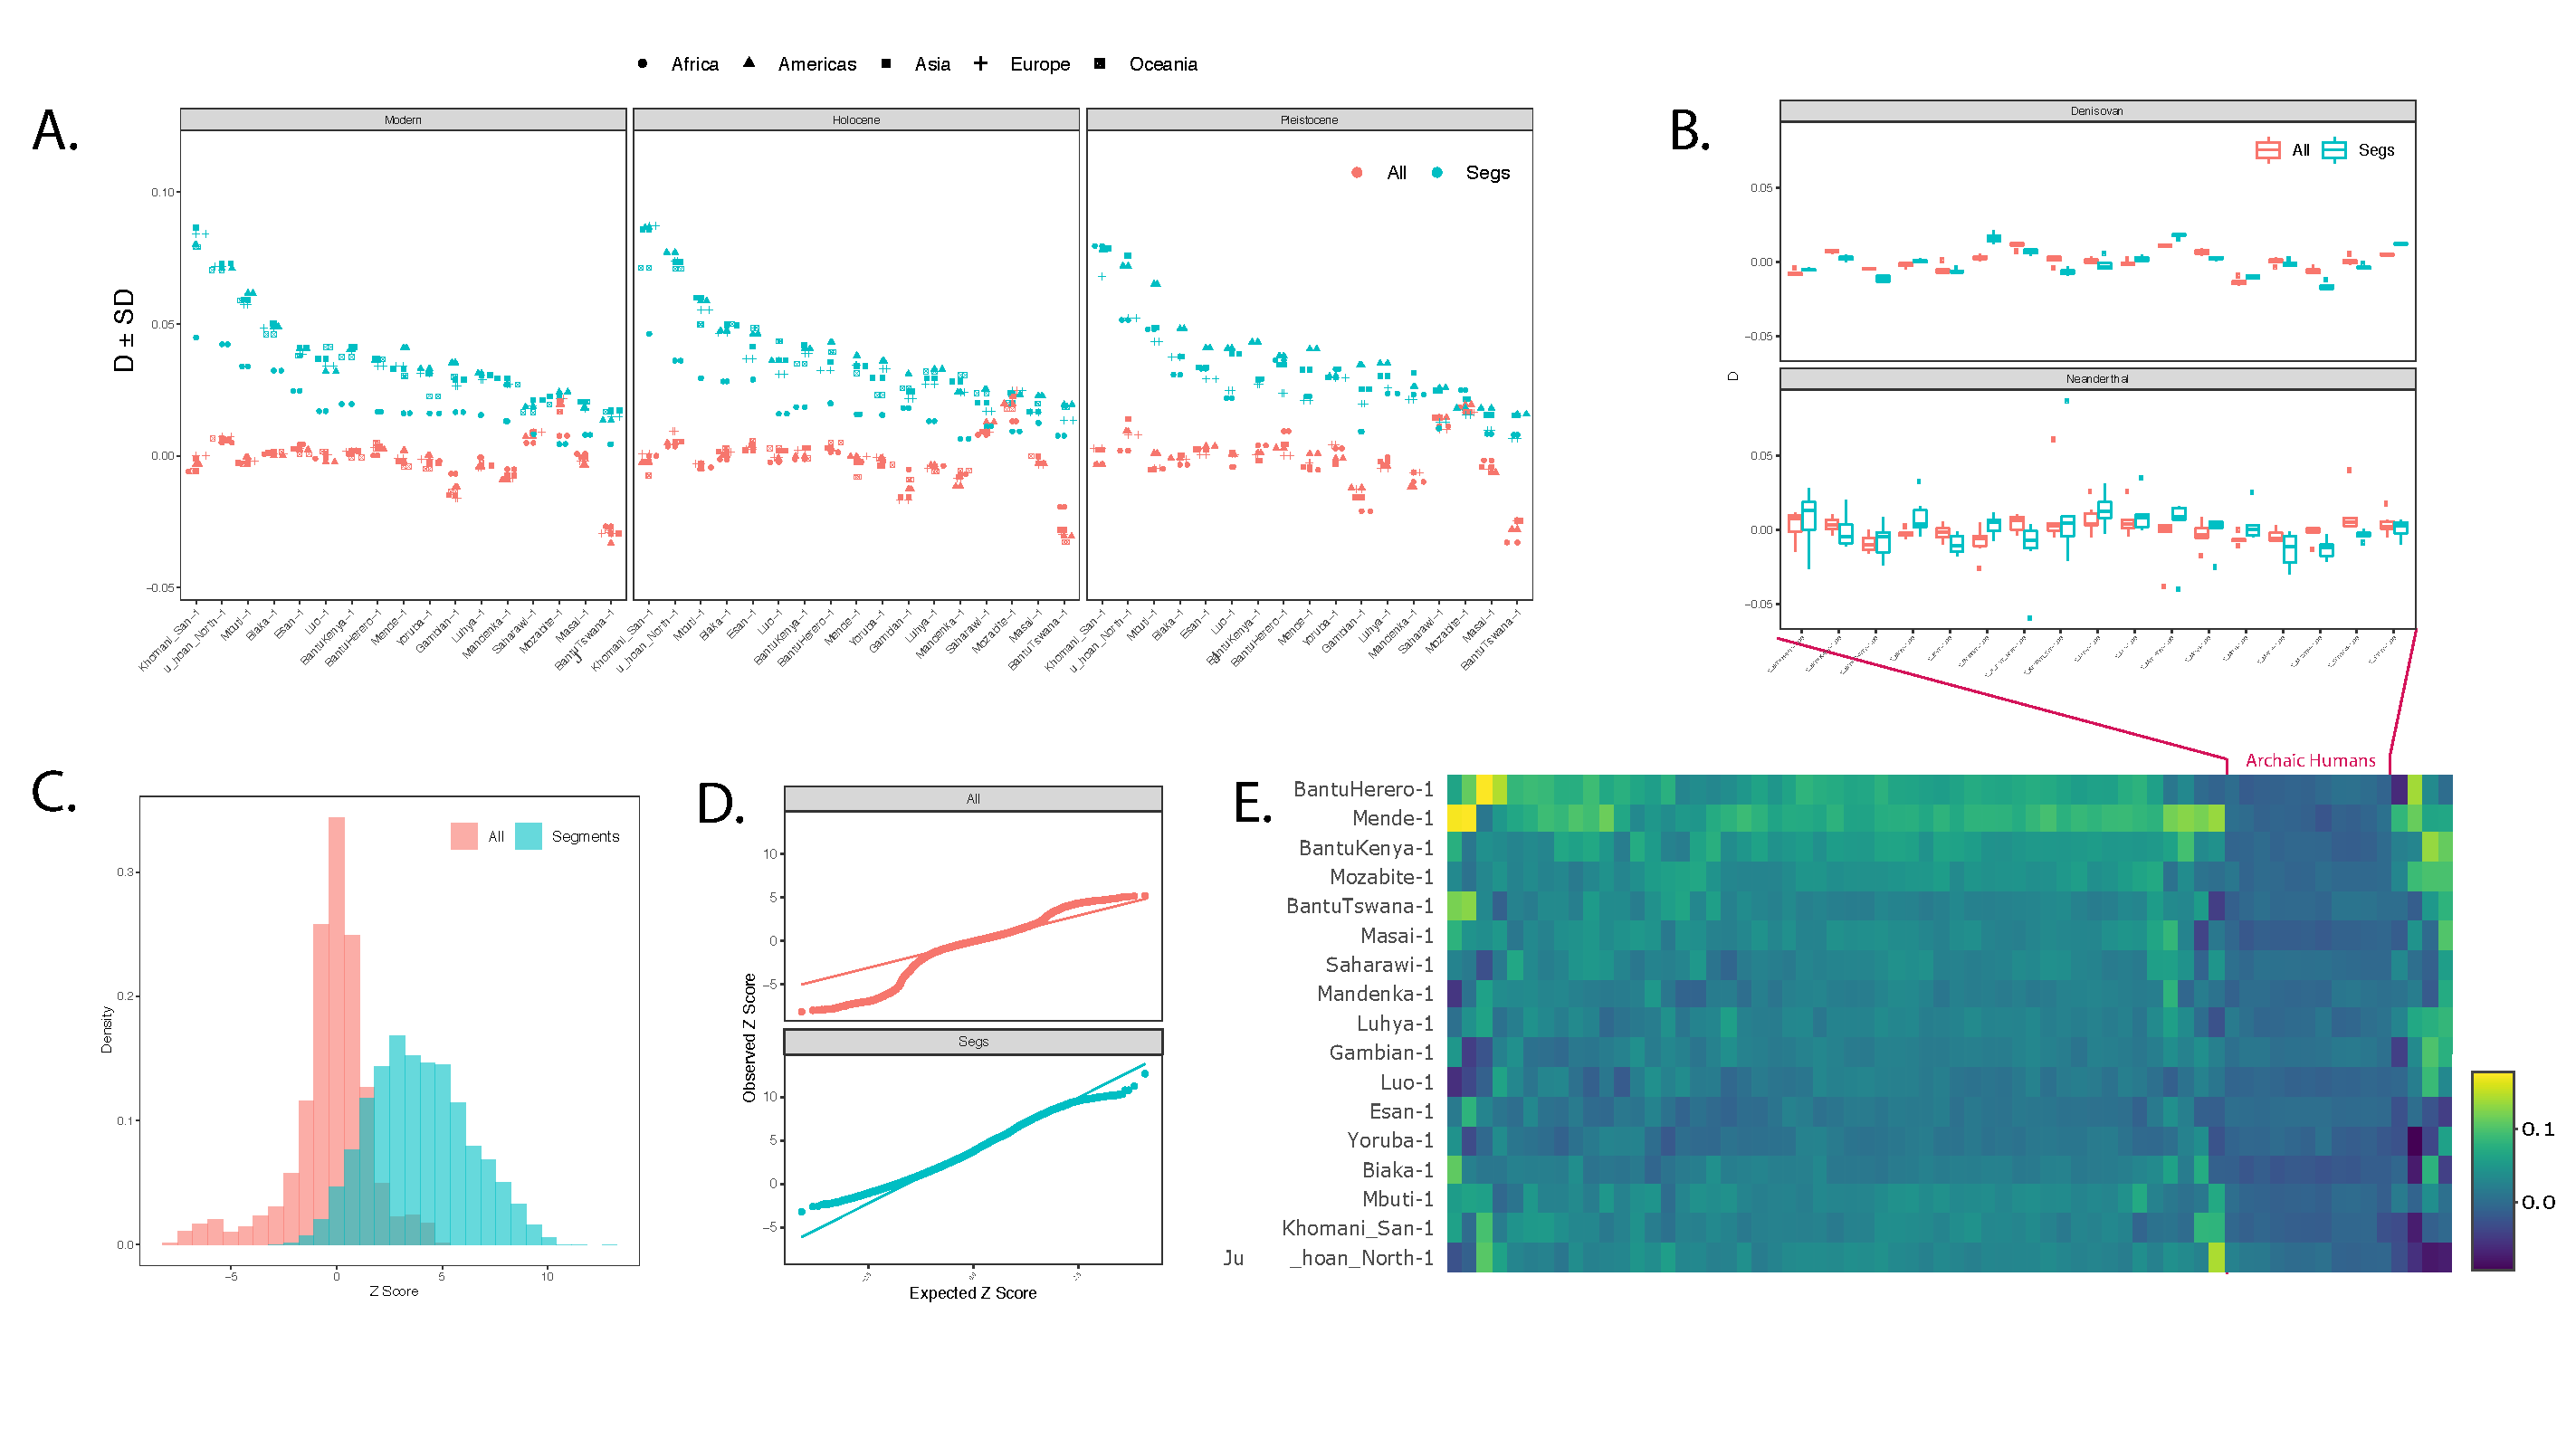
\includegraphics[width=\textwidth]{../plot/dstats.pdf}
	\caption{blah}
\end{figure}
\newpage

%\subsection*{URLs}
%\paragraph{Simons Genome Diversity Panel Phased Release} \url{https://sharehost.hms.harvard.edu/genetics/reich_lab/sgdp/phased_data/}
%\paragraph{Human Genome Diversity Panel} \url{ftp://ngs.sanger.ac.uk/production/hgdp/hgdp_wgs.20190516/}
%\paragraph{Ancient DNA} \url{http://cdna.eva.mpg.de/neandertal/}
%\paragraph{Strict 1000 Genomes Accessibility Mask} \url{ftp://ftp.1000genomes.ebi.ac.uk/vol1/ftp/release/20130502/supporting/accessible_genome_masks/}
%\paragraph{SMCSMC Implementation} \url{https://github.com/luntergroup/smcsmc}
%\paragraph{vcf2eigenstrat} \url{https://github.com/bodkan/vcf2eigenstrat}
%\paragraph{ADMIXTOOLS} \url{https://github.com/DReichLab/AdmixTools}
%\paragraph{admixr} \url{https://github.com/bodkan/admixr}


\newpage
\setcounter{section}{0}
\renewcommand{\thesection}{S\arabic{section}}%
\setcounter{table}{0}
\renewcommand{\thetable}{S\arabic{table}}%
\setcounter{figure}{0}
\renewcommand{\thefigure}{S\arabic{figure}}%

\section{Analysis of Simons Genome Diversity Panel}

We download variant call format (VCF) whole genome sequence (WGS) data from the phased release of the Simons Genome Diversity Panel and convert it to seg file format using a utility provided by the {\tt smcsmc} software implementation ({\tt smcsmc.vcf\_to\_seg}). We apply two masks to the data. Firstly, we mask the data with the strict accesibility mask provided by the 1000 genomes project (see URLs). Secondly, we mask any sites absent chimpanzee ancestry, due to a known issue in calling which resulted in artificially long runs of homozygosity. We develop a {\tt snakemake} pipeline for efficiently analysing sequence data with both {\tt smcsmc} and MSMC, available at the project's github page (see URLs). We assume a mutation rate of $1.25\times10^{-8}$ and a recombination rate of $3\times10^{-9}$, in line with recent literature. Two parameters must be set on a run-by-run basis. As the inference portion of {\tt smcsmc} uses a variational Bayesian approach, a number of maximum epochs must be set. Additionally, the number of particles to be used must be specified. All of the following analyses were run three times. 

We select one individual from each of the African populations in the SGDP and model their effective population size using both {\tt smcsmc} and MSMC (Figure \ref{sgdp_ne}). We simultaneously estimate directional migration rates in either direction with {\tt smcsmc}, with the converged solution representing a joint optimisation. Overall, both estimates are relatively consistent, especially in the estimation of the Eurasian $N_e$. However, in all cases, MSMC finds a higher African $N_e$ than does {\tt smcsmc} in the ancient past ($>$ 100kya). We expect that this is due to {\tt smcsmc} simultaneously estimating a high migration rate during this period in most of the African groups (Figure \ref{sgdp_mig}). A more thorough discussion of the discrepencies in effective population size estimates may be found in the main text. There are several interesting trends apparent in the estimated migration rates. Firstly, it appears that in almost all cases, the migration rate from African to Eurasian population exceeds that in the opposite direction. Secondly, the qualatative trends appear to break down by language phyla. Afroasiatic populations appear to have a large amount of migration in either direction, which is consistent with the literature. [TD1] Niger-Kordofanian and Nilo-Saharan populations appear to have comparable levels of migration at comparable times, approximatley peaking at between 2.5-3.0$\times 10^{-4}$ 40-70kya. Khoesan populations have a much lower level of migration, around 1$\times 10^{-4}$, though the timing of the peak is consistent with other groups. We wish to find the total fraction of a particular population replaced during a particular time period. We track the probability that a particular individual has not migrated after time $T$ (in generations). Let $\rho(t)$ be the instantaneous rate of migration per unit of time. In this formulation, $\frac{d}{dt} F(t) = - \rho(t) F(t)$, whose solution is $F(t) = e^{- \int_{t=0}^T \rho(t) dt}$; this gives a total migration probability in a range of epochs $E$ of  $1-F(T) = 1 - e^{\sum_{i \in E} r_i}$. We use this formulation to integrate all migration in the last 100ky (Figure \ref{sgdp_heatmap}). Even from a very abstracted statistic, Khoesan populations cluster distinctly at the extreme low end of migration, with Mbuti and Biaka (anciently diverged Pygmy populations) showing a transitional migration rate. Afroasiatic populations such as the Saharawi, Mozabite, and Somali show a qualitatively higher migration from Han and French than from Papuans, indicating recent admixture. 

To ensure that these results are reliable, we replicate our analysis in a subset of the HGDP which has been physically phased. This will additionally confirm that such trends are not the result of errors made during statistical phasing.

\begin{figure}
	\centering
	\label{sgdp_ne}
	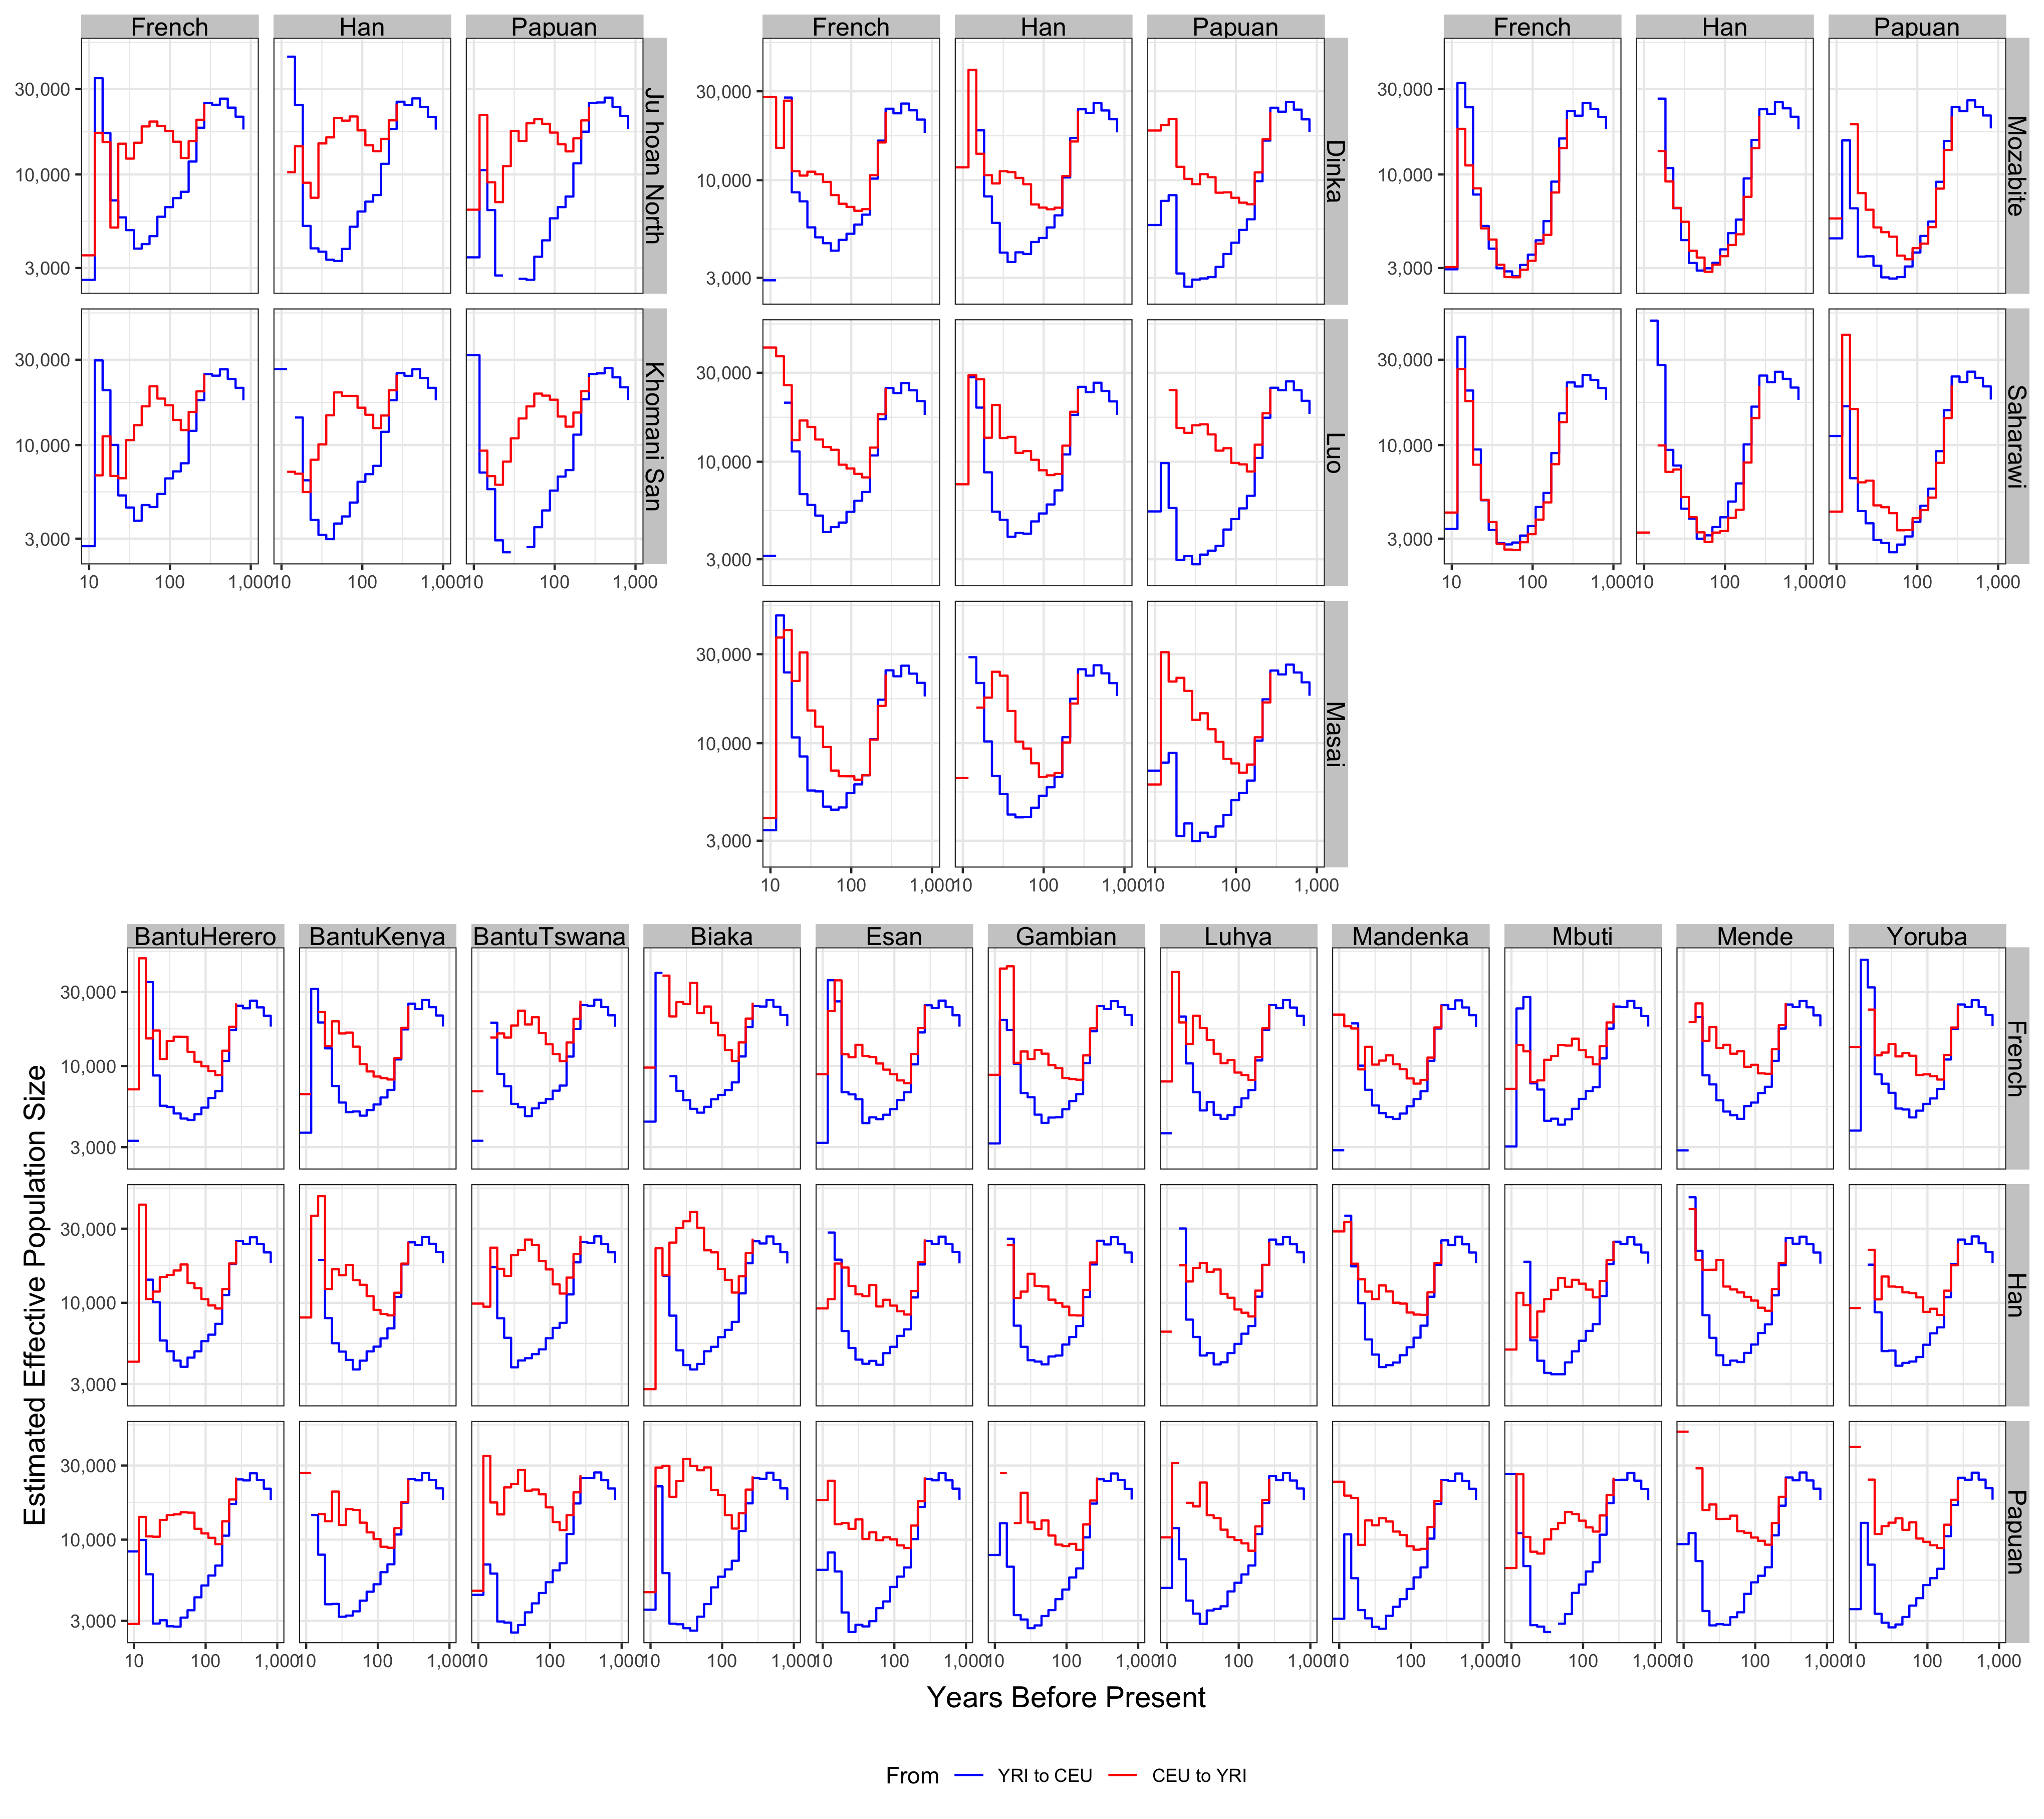
\includegraphics[width=\linewidth]{../plot/sgdp_ne.png}
	\caption{Estimated effective population size in different African and Eurasian groups with {\tt smcsmc}. 5000 particles and 10 variational Bayes interations were used to achieve convergence.}	
\end{figure}

\begin{figure}
	\centering
	\label{sgdp_mig}
	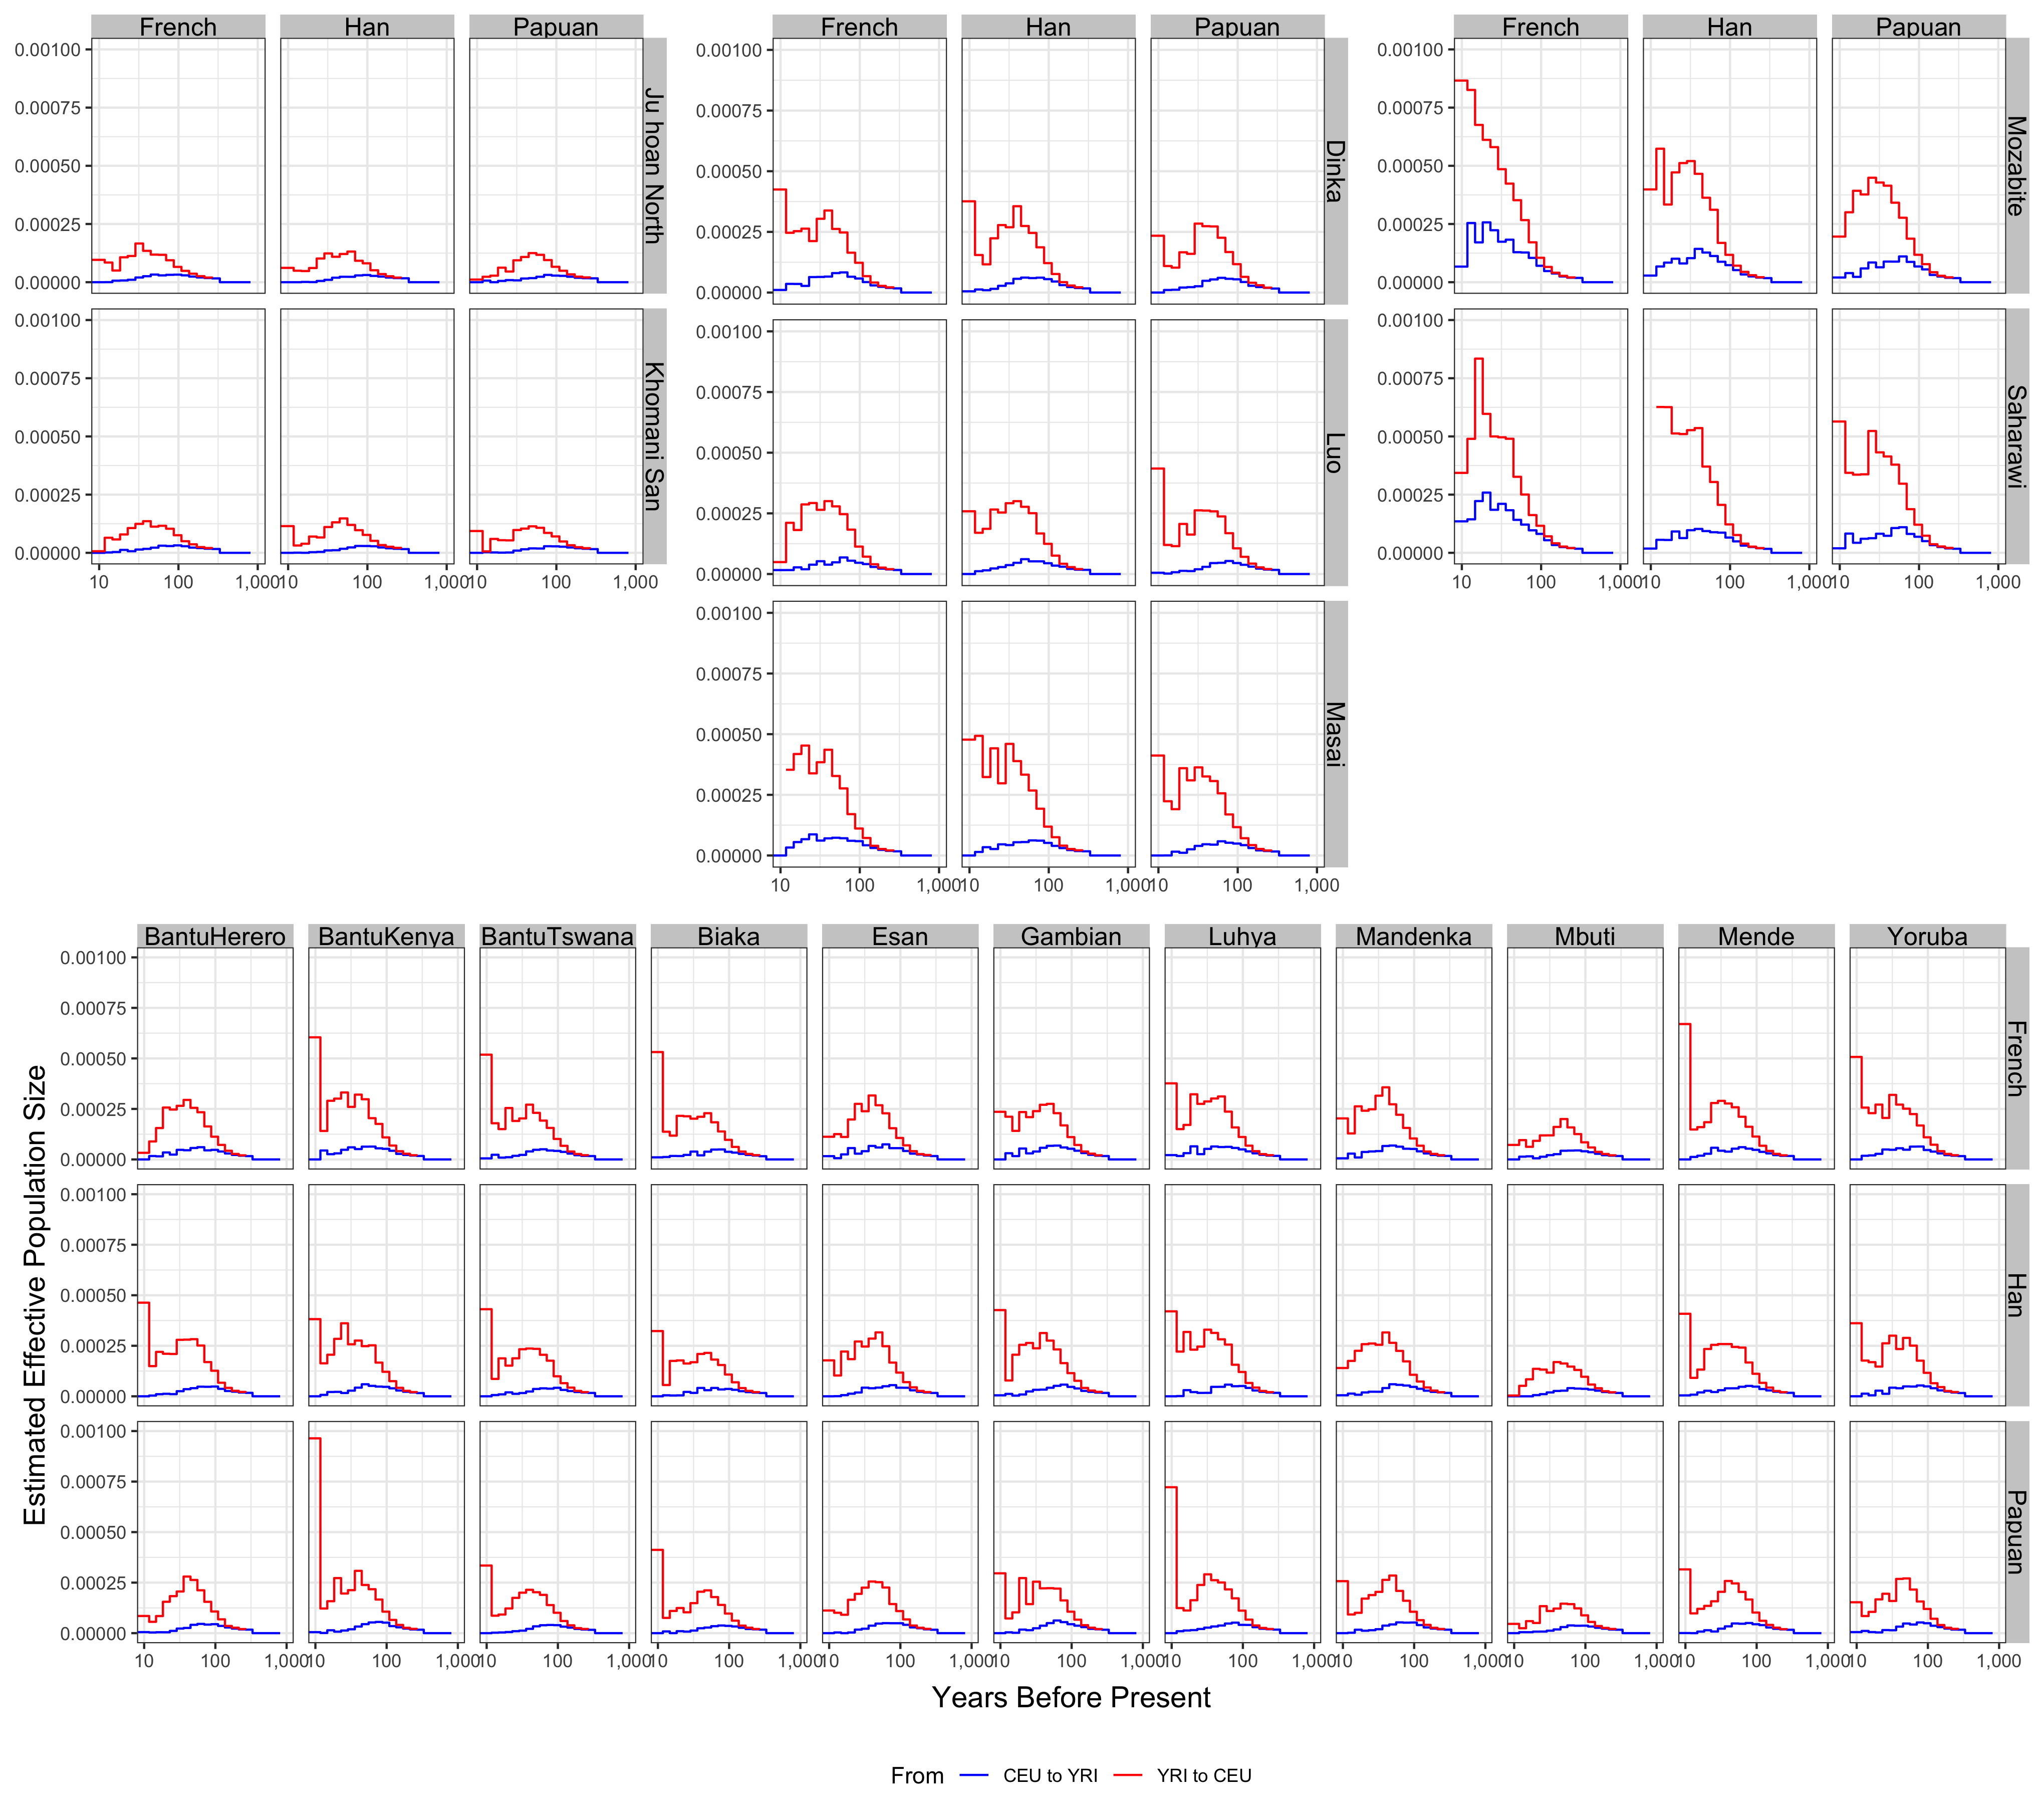
\includegraphics[width=\linewidth]{../plot/sgdp_mig.png}
	\caption{Estimated directional migration between African and Eurasian groups in the SGDP with {\tt smcsmc}. 5000 particles and 10 variational Bayes interations were used to achieve convergence.}	
\end{figure}

\begin{figure}
	\centering
	\label{sgdp_heatmap}
	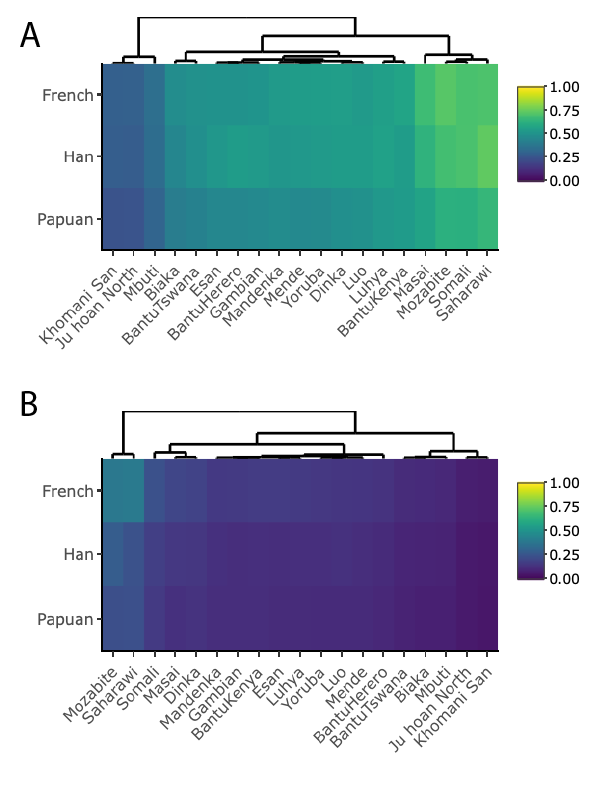
\includegraphics[width=\textwidth]{../plot/sgdp_heatmap.png}
	\caption{Integrated migration proportion in {\tt smcsmc} analysed SGDP populations.}
\end{figure}


\begin{enumerate}
    \item Whole analysis
    \item HGDP 
    \item HGDP subset in SGDP
\end{enumerate}

To directly compare these results to those obtained in the SGDP, we select the closest matching samples to those in the physically phased HGDP dataset and analyse these with MSMC and {\tt smcmsc} using 10k particles and 25 iterations to achieve convergence (Figure \ref{hgdp_sgdp_ne}). The effective sample size around the OoA migration is similarly inflated in MSMC analyses, while the estimation of the Eurasian population size remains largely consistent.  

\begin{figure}
    \centering
    \label{hgdp_sgdp_ne}
    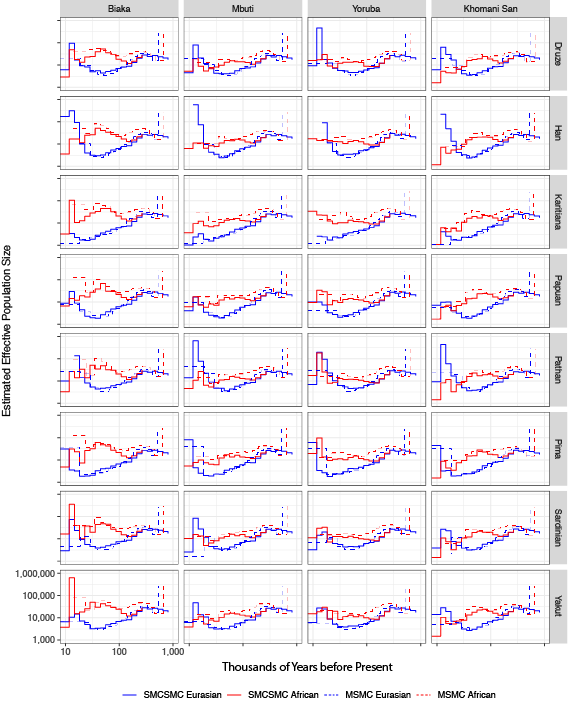
\includegraphics[width=\linewidth]{../plot/sgdp_subset_ne.png}
    \caption{{\tt smcsmc} and MSMC inferred effective population size of several populations in the Simons Genome Diversity Panel. These samples were selected to match, as closely as possible, those in the physically phased subet of the Human Genome Diversity Project panel. 10,000 particles and 25 iterations were used for {\tt smcsmc} and 40 iterations for MSMC.}
\end{figure}

\section{Statistical Analysis of Migrated Segments} \label{dstats}


\begin{enumerate}
	\item 
\end{enumerate}

\section{Simulation procedure} \label{sim}
\section{Population size simulations} \label{ne}
\section{Choice of initiation parameters} \label{minit}


\end{document}
